% Copyright 2021 Joel Feldman, Andrew Rechnitzer and Elyse Yeager, except where noted.
% This work is licensed under a Creative Commons Attribution-NonCommercial-ShareAlike 4.0 International License.
% https://creativecommons.org/licenses/by-nc-sa/4.0/


 \begin{frame}{Table of Contents }
\mapofcontentsA{\al,\atool}
 \end{frame}
%----------------------------------------------------------------------------------------

%----------------------------------------------------------------------------------------
\section{1.12  Improper Integrals}
%----------------------------------------------------------------------------------------
\begin{frame}
An integral is \alert{improper} if one or both of the following happen:
\begin{itemize}
	\item The region of integration is unbounded, e.g. $\int_1^\infty \frac{\sin x}{x} \ \dee x$\\
	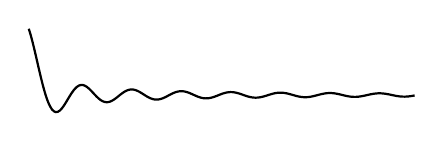
\begin{tikzpicture}
	\myaxis{...}{.2}{5}{}{1}{1}
	\draw[thick] plot[domain=1:50,xscale=0.1,smooth,samples=200](\x,{(sin (\x r))/\x});
	\end{tikzpicture}\pause $\Delta x = \frac{b-a}{n}=\frac{\infty}{n}$ ???\pause\hfill
	\item The integrand is unbounded over the interval, e.g. $\int_{-1}^1\frac1{x^2} \ \dee x$
	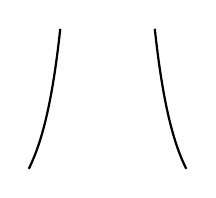
\begin{tikzpicture}
	\myaxis{}{1}{1}{}{0.2}{3}
	\draw[thick] plot[domain=-1:-.6](\x,{1/(\x*\x)});
	\draw[thick] plot[domain=.6:1](\x,{1/\x/\x});
	\end{tikzpicture}\pause\hfill $f(0)\Delta x=$  ???
	\end{itemize}
\unote{Definition~\eref{text}{def_improp_int}}
\end{frame}
%----------------------------------------------------------------------------------------
\begin{frame}\begin{block}{Strategy}
In both cases, we eliminate the offending parts of the integral using limits.\end{block}\vfill

$\displaystyle\int_1^{\alert\infty} \frac{\sin x}{x}\ \dee x = \sonslide<2->{\lim_{\alert b \to \infty}\left[\int_1^{\alert{b}} \frac{\sin x}{x}\ \dee x\right]}$
\vfill

$\displaystyle\int_{\alert0}^3 \frac1x\ \dee x = \sonslide<2->{\lim_{\alert a\to 0^+}\left[\int_{\alert a}^3\frac1x\ \dee x\right]}$
\vfill
If the limit doesn't exist, we say the integral \alert{diverges}. Otherwise it \alert{converges}.
\end{frame}
%----------------------------------------------------------------------------------------

%\subsection{Type 1: unbounded region of integration}
%----------------------------------------------------------------------------------------
\begin{frame}[t]
\nsAnswerYes<1>
\AnswerYes<1>
\begin{align*}
\int_1^\infty \frac1x\ \dee x&=\onslide<2-|handout:0>{
	\lim_{a \to \infty}\left[\int_1^a\frac1x\ \dee x\right]\\
	&=\lim_{a \to \infty}\left[\log a \right]=
	\infty}
\end{align*}
\color{spoilercolor}
\pause
\onslide<+-|handout:0>{We say this integral \alert{diverges} because the limit is not a number.
	\begin{tikzpicture}
	\myaxis{x}{0}{10}{y}{0}{2}
	\draw[thick] plot[domain=.5:10,smooth, samples=50] ({\x},{1/\x});
	\xcoord{1}{1}
	
	\onslide<+>{
		\fill[opacity=0.5,left color=C1, right color=C5] (1,0)--(1,1) plot[domain=1:2](\x,1/\x)--(2,0)--(1,0);
		\xcoord{2}{2}
		\draw (1.5,-1) node{$A\approx 0.7$};
	}
	
	\onslide<+>{
		\fill[opacity=0.5,left color=C1, right color=C5] (1,0)--(1,1) plot[domain=1:3](\x,1/\x)--(3,0)--(1,0);
		\xcoord{3}{4}
		\draw (2,-1) node{$A\approx 1.4$};
	}
	
	\onslide<+>{
		\fill[opacity=0.5,left color=C1, right color=C5] (1,0)--(1,1) plot[domain=1:6](\x,1/\x)--(6,0)--(1,0);
		\xcoord{6}{10}
		\draw (3.5,-1) node{$A\approx 2.3$};
	}
	
	\onslide<+>{
		\fill[opacity=0.5,left color=C1, right color=C5] (1,0)--(1,1) plot[domain=1:9](\x,1/\x)--(9,0)--(1,0);
		\xcoord{9}{100}
		\draw (4,-1) node{$A\approx 4.6$};
	}
	
	\onslide<+>{
		\fill[opacity=0.5,left color=C1, right color=C5] (1,0)--(1,1) plot[domain=1:9.75](\x,1/\x)--(9.75,0)--(1,0);
		\xcoord{9.75}{1000}
		\draw (4.5,-1) node{$A\approx 6.9$};
	}
	
		\onslide<+->{
		\fill[opacity=0.5,left color=C1, right color=C5] (1,0)--(1,1) plot[domain=1:10](\x,1/\x)|-(1,0);}
\onslide<8>{ \draw (4.5,-1) node{$A\approx 1000$};}	
\onslide<9>{		\draw (4.5,-1) node{$A\approx 1000000$};}	
\onslide<10>{		\draw (4.5,-1) node{$A\approx 1000000000000$ etc};}	
	\end{tikzpicture}
}
\StatusBar{2}{10}
\end{frame}
%----------------------------------------------------------------------------------------
%----------------------------------------------------------------------------------------
%----------------------------------------------------------------------------------------
\begin{frame}[t]
\nsAnswerYes<1>
\AnswerYes<1>
\begin{align*}
\int_1^\infty \frac1{x^2}\ \dee x&=\onslide<2-|handout:0>{
	\lim_{a \to \infty}\left[\int_1^a\frac1{x^2}\ \dee x\right]\\
	&=\lim_{a \to \infty}\left[-\frac{1}{a}+1 \right]=1
}
\end{align*}
\color{spoilercolor}
\pause
\onslide<+-|handout:0>{We say this integral \alert{converges} because the limit is  a number.
	\begin{tikzpicture}
	\myaxis{x}{0}{10.1}{}{0}{2}
	\draw[thick] plot[domain=.7:10,smooth, samples=50] ({\x},{1/(\x*\x)});
	\xcoord{1}{1}
	
	\onslide<+>{
		\fill[opacity=0.5,left color=C1, right color=C5] (1,0)--(1,1) plot[domain=1:2](\x,{1/(\x*\x)})--(2,0)--(1,0);
		\xcoord{2}{2}
		\draw (2,1) node{$A= 0.5$};
	}
	
	\onslide<+>{
		\fill[opacity=0.5,left color=C1, right color=C5] (1,0)--(1,1) plot[domain=1:3](\x,{1/(\x*\x)})--(3,0)--(1,0);
		\xcoord{3}{4}
		\draw (2,1) node{$A= 0.75$};
	}
	
	\onslide<+>{
		\fill[opacity=0.5,left color=C1, right color=C5] (1,0)--(1,1) plot[domain=1:6](\x,{1/(\x*\x)})--(6,0)--(1,0);
		\xcoord{6}{10}
		\draw (3.5,1) node{$A=0.9$};
	}
	
	\onslide<+>{
		\fill[opacity=0.5,left color=C1, right color=C5] (1,0)--(1,1) plot[domain=1:9](\x,{1/(\x*\x)})--(9,0)--(1,0);
		\xcoord{9}{100}
		\draw (4,1) node{$A=0.99$};
	}
	
	\onslide<+->{
		\fill[opacity=0.5,left color=C1, right color=C5] (1,0)--(1,1) plot[domain=1:9.75](\x,{1/(\x*\x)})--(9.75,0)--(1,0);
		
	}
\onslide<7>{	\xcoord{9.75}{1000}\draw (4.5,1) node{$A=0.999$};}
\onslide<8>{		\draw (4.5,1) node{$A=0.999999$};}
\onslide<9>{		\draw (4.5,1) node{$A=0.999999999$ etc};}
\end{tikzpicture}
}\StatusBar{2}{9}
\end{frame}

%\subsection{Multiple Regions}
%----------------------------------------------------------------------------------------
\begin{frame}[t]
\MoreSpace<1>
\StatusBar{3}{10}
Evaluate $\displaystyle\int_{-\infty}^\infty \frac{1}{1+x^2}\ \dee x$

\only<1>{When an integral has multiple sources of impropriety, we break it up into integrals that have only one source each. If all of them converge, the original integral converges. If any of them diverges, the original integral diverges as well.}

\sonslide<3->{
\begin{align*}
&=\textcolor{W1}{\int_{-\infty}^0 \frac{1}{1+x^2}\ \dee x}+\int_0^{\infty} \frac{1}{1+x^2}\ \dee x\\
\onslide<3-|handout:0>{
	&=\textcolor{W1}{\lim_{a \to -\infty}\left[\int_a^0\frac{1}{1+x^2}\ \dee x\right]}+
	\lim_{b \to \infty}\left[\int_0^b\frac{1}{1+x^2}\ \dee x\right]\\
	&=\textcolor{W1}{\lim_{a \to -\infty}\left[\arctan 0 - \arctan a\right]}+
	\lim_{b \to \infty}\left[\arctan b - \arctan 0\right]\\
	&=\textcolor{W1}{\frac{\pi}{2}}+\frac{\pi}{2}=\pi
}
\end{align*}}
\onslide<3-|handout:0>{\color{spoilercolor}
	\begin{tikzpicture}
	
	\myaxis{x}{5.1}{5.1}{}{0}{2}
	\draw[thick] plot[domain=-5:5,smooth, samples=50] ({\x},{1/(\x*\x+1)});
	
	
	\onslide<4>{
		\fill[opacity=0.5,left color=C1, right color=C5] (0,0)--(0,1) plot[domain=0:1](\x,{1/(\x*\x+1)})--(1,0)--(0,0);
		\xcoord{1}{1}
		\draw (1,1) node{$A\approx \frac{\pi}{2}-0.8$};
		
	}
	
	\onslide<5>{
		\fill[opacity=0.5,left color=C1, right color=C5] (0,0)--(0,1) plot[domain=0:2](\x,{1/(\x*\x+1)})--(2,0)--(0,0);
		\xcoord{2}{2}
		\draw (2,1) node{$A\approx \frac{\pi}{2}-0.5$};
		
	}
	
	\onslide<6>{
		\fill[opacity=0.5,left color=C1, right color=C5] (0,0)--(0,1) plot[domain=0:3](\x,{1/(\x*\x+1)})--(3,0)--(0,0);
		\xcoord{3}{3}
		\draw (3,1) node{$A\approx \frac{\pi}{2}-0.3$};
		
	}
	
	\onslide<7>{
		\fill[opacity=0.5,left color=C1, right color=C5] (0,0)--(0,1) plot[domain=0:4](\x,{1/(\x*\x+1)})--(4,0)--(0,0);
		\xcoord{4}{4}
		\draw (4,1) node{$A\approx \frac{\pi}{2}-0.25$};
		
	}
	
	\onslide<8>{
		\fill[opacity=0.5,left color=C1, right color=C5] (0,0)--(0,1) plot[domain=0:4.75](\x,{1/(\x*\x+1)})--(4.75,0)--(0,0);
		\xcoord{5}{100}
		\draw (4.5,1) node{$A\approx \frac{\pi}{2}-0.01$};
	}
	\onslide<9->{
		\fill[opacity=0.5,left color=C1, right color=C5] (0,0)--(0,1) plot[domain=0:5](\x,{1/(\x*\x+1)})--(5,0)--(0,0);
		\draw (5,1) node{$A_1= \frac{\pi}{2}$};
	}
	
	\onslide<10->{
		\fill[opacity=0.5,left color=W1, right color=W5] (0,0)--(0,1) plot[domain=0:-5](\x,{1/(\x*\x+1)})--(-5,0)--(0,0);
		\draw (-5,1) node[W1]{$A_2= \frac{\pi}{2}$};
	}
	\end{tikzpicture}
}
\end{frame}


%----------------------------------------------------------------------------------------
%----------------------------------------------------------------------------------------
%\subsection{Type 2: unbounded integrand}

%----------------------------------------------------------------------------------------
\begin{frame}[t]
\begin{multicols}{2}
	Evaluate $\displaystyle\int_{0}^1 \frac{1}{2\sqrt x}\ \dee x$\\ \vfill
	
	\sonslide<3->{Same idea: we solve our problems by ignoring them (temporarily).\\
		Eliminate the problematic part of the integral using a limit.}
	
	\columnbreak
	
	\onslide<2->{\begin{tikzpicture}
		\myaxis{x}{0}{4}{}{0}{4}
		\draw[thick] plot[domain=.25:3.75,smooth]({1/(4*\x*\x)},{\x});
		\xcoord{1}{1}
		
		\sonslide<2-3>{
			\fill[opacity=0.5,left color=W3, right color=W1]  plot[domain=.5:3.75]({1/(4*\x*\x)},{\x})--(0,4)--(0,0)--(1,0);
		}
		
		\snshonslide{5-7}{2}{0}{
			\fill[opacity=0.5,left color=W3, right color=W1]  plot[domain=.5:1]({1/(4*\x*\x)},{\x})|-(1,0);
			\xcoord{.25}{a}
			\sonslide<7>{\draw (1.25,1)node{$A\approx 0.5$};}
		}
		
		\snshonslide{8}{3}{0}{
			\fill[opacity=0.5,left color=W3, right color=W1]  plot[domain=.5:1.41]({1/(4*\x*\x)},{\x})|-(1,0);
			\xcoord{.125}{a}
			\draw (1.25,1)node{$A\approx 0.6$};
		}
		
		\snshonslide{9}{4}{0}{
			\fill[opacity=0.5,left color=W3, right color=W1]  plot[domain=.5:3]({1/(4*\x*\x)},{\x})|-(1,0);
			\xcoord{.03}{a}
			\draw (1.25,1)node{$A\approx 0.8$};
		}
		
		\snshonslide{10}{5}{0}{
			\fill[opacity=0.5,left color=W3, right color=W1]  plot[domain=.5:4]({1/(4*\x*\x)},{\x})|-(1,0);
			\xcoord{.01}{a}
			\draw (1.25,1)node{$A\approx 0.999$};
		}
		
		\end{tikzpicture}}
\end{multicols}
\sonslide<4->{
	\[
	\int_{0}^1 \frac{1}{2\sqrt x}\ \dee x=\lim_{a \to 0^+}\left[\int_a^1 \frac1{2\sqrt x}\ \dee x
	\right]
	\onslide<6->{
		=\lim_{a\to 0^+}\left[1-\sqrt a \right]=1
	}
	\]
}
\sStatusBar{6}{10}
\nsStatusBar{2}{5}
\end{frame}


%----------------------------------------------------------------------------------------
%----------------------------------------------------------------------------------------
\begin{frame}[t]	
	Evaluate $\displaystyle\int_{-2}^1 \frac{1}{x^2}\ \dee x$

\sonly<2>{
	\begin{align*}
\int x^{-2}\ \dee x & =-x^{-1}+C=-\frac{1}{x}+C\\
\lim_{a \to 0^+}\int_{a}^1 \frac{1}{x^2}\ \dee x & =\lim_{a \to 0^+}\left[-\frac1x\right]_a^1\\
&=\lim_{a \to 0^+}\left[-1+\frac1a\right]=\infty
\end{align*}
Once we see that one part of the improper integral diverges, we stop: the entire integral diverges, regardless of what happens to the left of the $y$-axis.
	}

\snshonslide{3-}{2-}{0}{
	\hspace{1cm}
	\begin{tikzpicture}[yscale=.6]
	\myaxis{x}{4}{4}{}{0}{10}
	\draw[thick] plot[domain=.316:4,smooth](\x,{1/(\x*\x)});
	\draw[thick] plot[domain=-4:-.316,smooth](\x,{1/(\x*\x)});
	
	\xcoord{1}{1}
	\xcoord{-2}{-2}
	
	%%big steps, positive half of axis
	\foreach \x[evaluate=\sl using int(\x-1)] in {4,5}{
		\onslide<\sl|handout:0>{
			%show area
			\DIVIDE{\x}{5}{\d}
			\SUBTRACT{1.4}{\d}{\a}
			\fill[opacity=0.5,left color=W3, right color=W1]  plot[domain=\a:1](\x,{1/(\x*\x)})--(1,0)-|cycle;
			\xcoord{\a}{a }
			
			%calculate area=num/denom=(x-2)(7-x)
			\SUBTRACT{\x}{2}{\num}
			\SUBTRACT{7}{\x}{\denom}
			\DIVIDE{\num}{\denom}{\area}
			%print area
			\ROUND[1]{\area}{\printarea}
			\draw (1,4)node[right]{$\int_a^1\frac{1}{x^2}\dee x\approx\printarea$};
	}}
	
	%smaller steps, positive half of axis
	\foreach \s in {5,6,7}{
		\onslide<\s|handout:0>{
			%show area
			\SUBTRACT{8}{\s}{\aa}
			\DIVIDE{\aa}{10}{\a} %a=(56-s)/100
			
			\begin{scope}\clip(0,0) rectangle (1.5,10);
			\fill[opacity=0.5,left color=W3, right color=W1]  plot[domain=\a:1](\x,{1/(\x*\x)})--(1,0)-|cycle;\end{scope}
			
			\xcoord{\a}{a}
			
			%calculate area=1/a-1
			\DIVIDE{1}{\a}{\t}
			\SUBTRACT{\t}{1}{\area}
			%print area
			\ROUND[1]{\area}{\printarea}
			\draw (1,4)node[right]{$\int_a^1\frac{1}{x^2}\dee x\approx\printarea$};
	}}
	
	\onslide<8|handout:0>{
		\begin{scope}\clip(0,0) rectangle (1.5,10);
		\fill[opacity=0.5,left color=W3, right color=W1]  plot[domain=0.05:1](\x,{1/(\x*\x)})--(1,0)-|cycle;\end{scope}
		
		\xcoord{0.05}{a}
		
		\draw (1,4)node[right]{$\int_a^1\frac{1}{x^2}\dee x\approx1\ 000\ 000$ etc};
}
	\end{tikzpicture}}
\StatusBar{2}{8}
\end{frame}

%----------------------------------------------------------------------------------------
%----------------------------------------------------------------------------------------
\begin{frame}[t]
Evaluate $\displaystyle\int_{0}^{\infty}\frac{\cos x}{1+\sin^2 x}\,\dee x$, or show that it diverges.

\sonslide<2->{
\begin{align*}
u&=\sin x,\ \dee u= \cos x\, \dee x\\
u(0)&=0\\
\lim_{b \to \infty}\left[\int_0^b \frac{\cos x}{1+\sin^2 x}\,\dee x\right]&=
\lim_{b \to \infty}\left[\int_0^{\sin b}\frac{1}{1+u^2}\,\dee u\right]
\\&=\lim_{b\to\infty}\left[\arctan(\sin b)-\arctan (0)\right]\\
&=\lim_{b\to\infty}\left[\arctan(\sin b)\right]
\end{align*}
As $b$ goes to infinity, $\sin b$ oscillates between $-1$ and $1$, so $\arctan (\sin b)$ oscillates between $-\frac{\pi}{4}$ and $\frac{\pi}{4}$. Since its limit does not exist, the integral \alert{diverges}.
}
\end{frame}

%----------------------------------------------------------------------------------------
\begin{frame}<beamer>
\StatusBar{1}{17}
\color{C1}

\begin{tikzpicture}
\myaxis{x}{0}{8.5}{y}{1.1}{1}
\draw[thick,C1] plot[samples=50,domain=0:8.5,smooth](\x,{cos(\x*3 r)/(1+sin(\x*3 r)*sin(\x*3 r))})node[right]{$y=\frac{\cos x}{1+\sin^2 x}$};
\foreach \s in {0,1,2,3}{
	\MULTIPLY{\s}{4}{\slide}
	\ADD{\slide}{2}{\slidea}
	\MULTIPLY{\s}{2.094}{\lx}%start of period: 2pi/3*s
	\ADD{\lx}{0.5236}{\mx}%move up pi/6 each time
	\ADD{\mx}{0.5236}{\nx}%move up pi/6 each time
	\ADD{\nx}{0.5236}{\ox}%move up pi/6 each time
	\ADD{\ox}{0.5236}{\px}%move up pi/6 each time
	
	\onslide<\slidea->{\fill[C2,opacity=0.2] plot[domain=\lx:\mx](\x,{cos(\x*3 r)/(1+sin(\x*3 r)*sin(\x*3 r))})-|cycle;}
	\onslide<\slidea>{\draw[|-|](0,-1.5)-- (\mx,-1.5)node[midway,below]{$A=\frac{\pi}{4}$};}
	
	\ADD{\slidea}{1}{\slideb}
	\onslide<\slideb->{\fill[M4,opacity=0.2] plot[domain=\mx:\nx](\x,{cos(\x*3 r)/(1+sin(\x*3 r)*sin(\x*3 r))})|-cycle;}
	\onslide<\slideb>{\draw[|-|](0,-1.5)-- (\nx,-1.5)node[midway,below]{$A=0$};}
	
	\ADD{\slideb}{1}{\slidec}
	\onslide<\slidec->{\fill[W1,opacity=0.2] plot[domain=\nx:\ox](\x,{cos(\x*3 r)/(1+sin(\x*3 r)*sin(\x*3 r))})-|cycle;}
	\onslide<\slidec>{\draw[|-|](0,-1.5)-- (\ox,-1.5)node[midway,below]{$A=-\frac{\pi}{4}$};}
	
	
	\ADD{\slidec}{1}{\slided}
	\onslide<\slided->{\fill[C1,opacity=0.2] plot[domain=\ox:\px](\x,{cos(\x*3 r)/(1+sin(\x*3 r)*sin(\x*3 r))})|-cycle;}
	\onslide<\slided>{\draw[|-|](0,-1.5)-- (\px,-1.5)node[midway,below]{$A=0$};}
	
	}
	\xcoord{3.14}{\pi}
	\xcoord{6.26}{2\pi}
	
\end{tikzpicture}
\end{frame}
%----------------------------------------------------------------------------------------
%----------------------------------------------------------------------------------------
\begin{frame}{Warning: Sneaky Divergence}
\only<1>{
If you don't realize that an integral diverges, you can generate answers that look plausible but are secretly nonsense.
\vfill

 For example, attempting to use the Fundamental Theorem of Calculus in the example $\ds\int_{-2}^1\frac{1}{x^2}\dee x$ gives $\ds\left[-\frac{1}{x}\right]_{-2}^1=-\frac32$: a poor approximation for positive infinity!}
\only<2-|handout:0>{
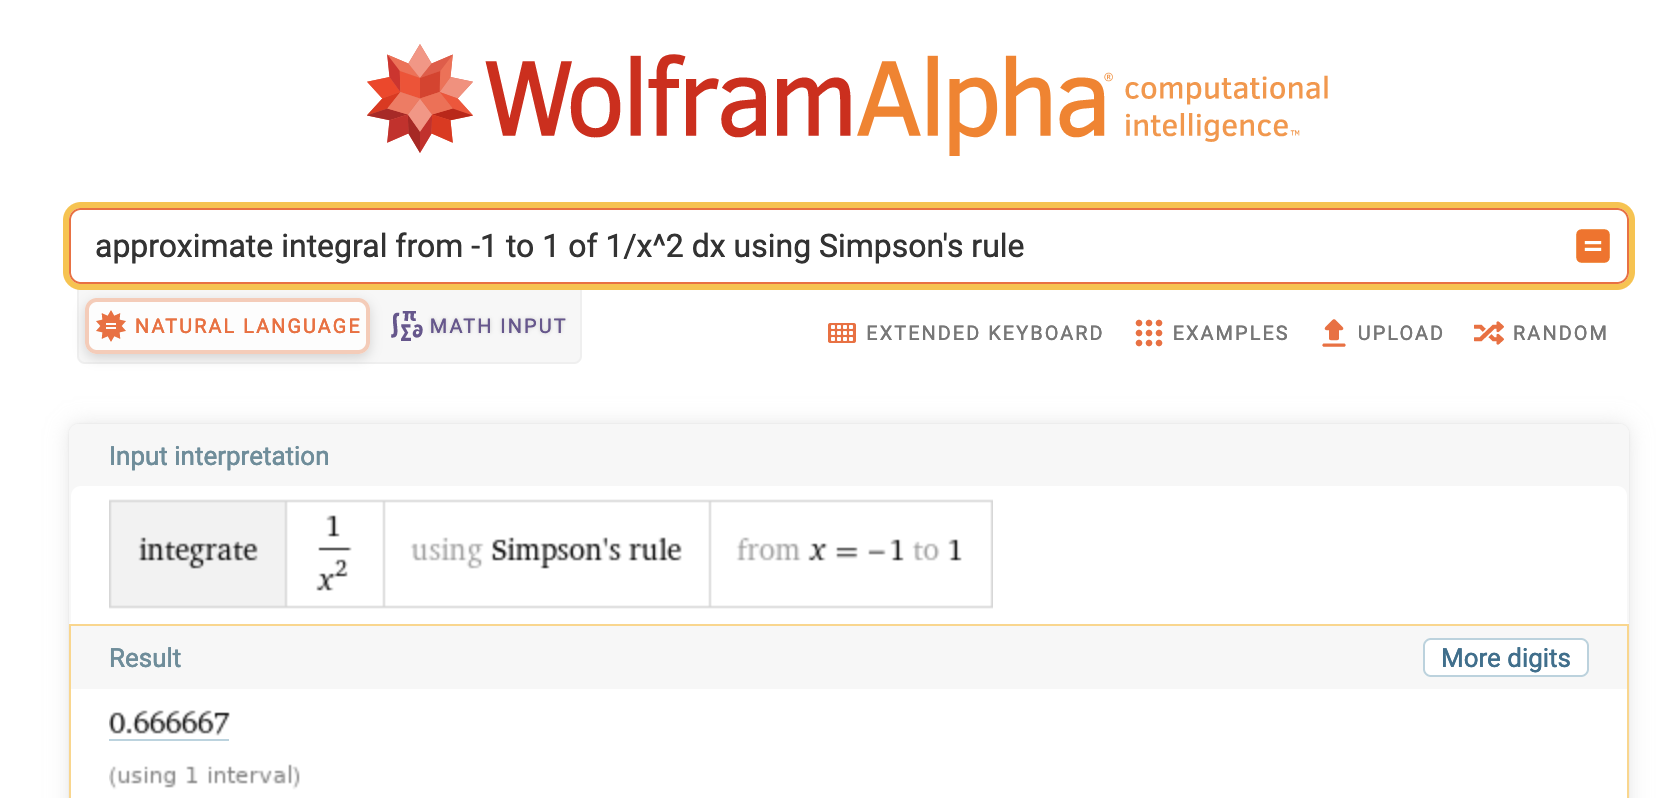
\includegraphics[height=4.5cm]{clipart/WA-divergent}
\index{
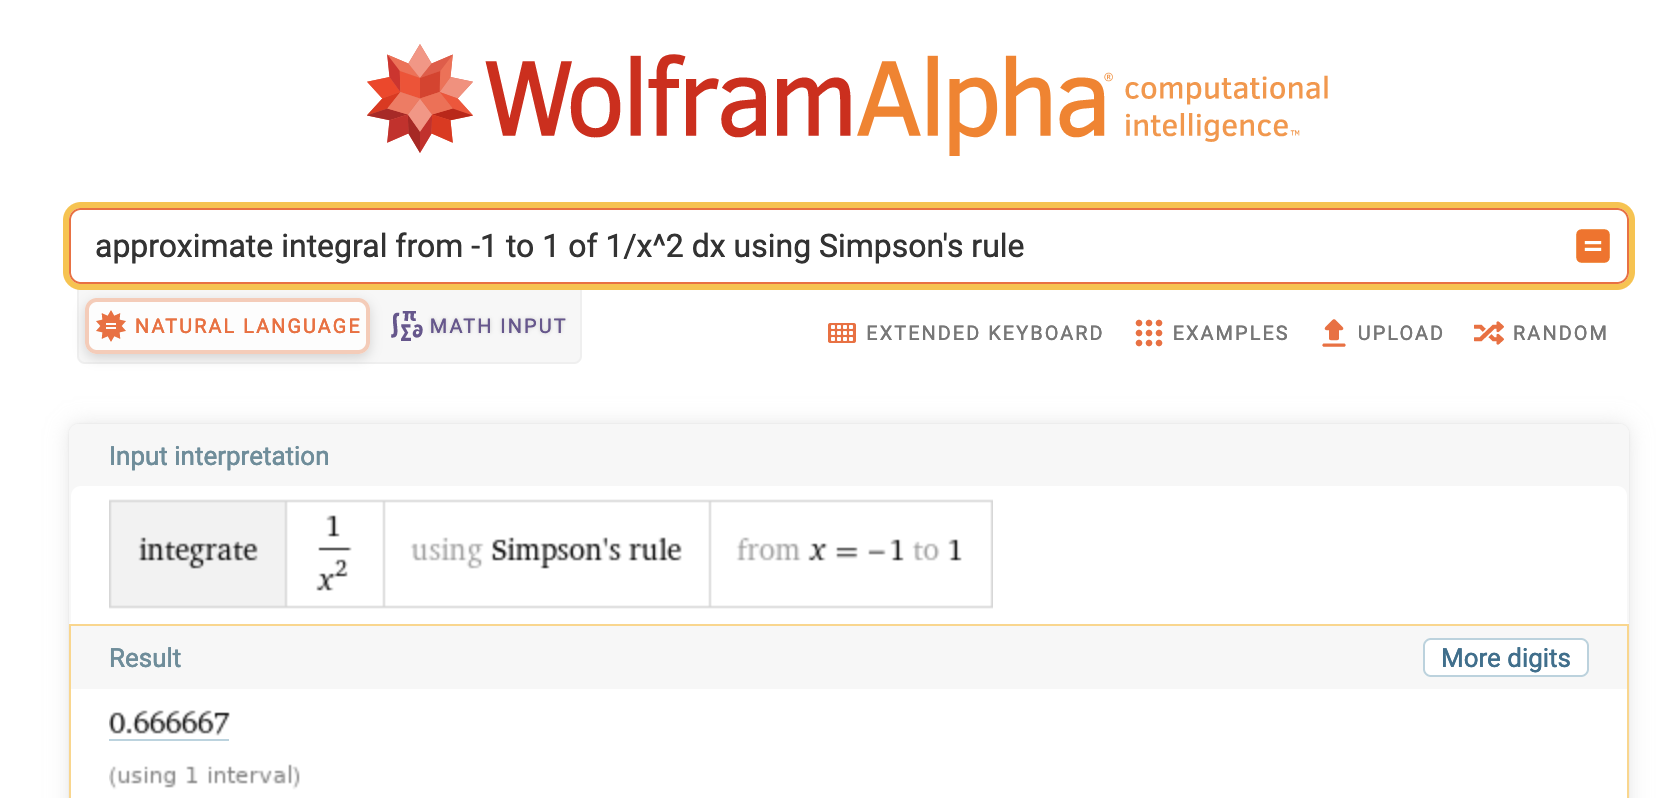
\includegraphics[height=3mm]{clipart/WA-divergent}
\href{https://www.wolframalpha.com/input/?i=approximate+integral+from+-0.1+to+0.2+of+1\%2Fx\%5E2+\dee x+using+Simpson\%27s+rule}{WolframAlpha (accessed 25 August 2021)}
}\vfill

This mistake can be especially dangerous using computer algebra systems, where you spend less time thinking about the integral and so have fewer chances to notice that something is awry. As of this writing, %\footnote{25 August 2021} 
\href{https://www.wolframalpha.com/input/?i=approximate+integral+from+-1+to+1+of+1\%2Fx\%5E2+dx+using+Simpson\%27s+rule}{WolframAlpha} gives no warnings when you ask it to approximate $\int_{-1}^1\frac{1}{x^2}\dee x$ using Simpson's Rule: it tells you the approximation with one parabola is $\frac23$.}
\end{frame}
%----------------------------------------------------------------------------------------

%----------------------------------------------------------------------------------------
%----------------------------------------------------------------------------------------
\begin{frame}[t]
\AnswerSpace\only<1>{\AnswerYes}
Evaluate $\displaystyle\int_0^1\frac1{x^p}\dee x$ and $\displaystyle\int_1^\infty\frac1{x^p}\dee x$
when $p$ is constant.

\sonslide<2->{
\begin{align*}
\int\frac{1}{x^p}\ \dee x &= \int x^{-p}\ \dee x=\begin{cases}
\log|x|+C & \mbox{ if } p=1\\
\frac{x^{1-p}}{1-p}+C & \mbox{ if } p\neq 1
\end{cases}\\
\int_a^b \frac{1}{x^p}\ \dee x & =\begin{cases}
\log|b|-\log|a| & \mbox{ if } p=1\\
\frac{b^{1-p}-a^{1-p}}{1-p} & \mbox{ if } p\neq 1
\end{cases}
\quad\text{if }x=0\text{ is not in }[a,b]\\
\int_1^\infty\frac{1}{x^p}\ \dee x & = \begin{cases}
\lim\limits_{b \to \infty}\log|b| & \mbox{ if } p=1\\
\lim\limits_{b \to \infty}\left[\frac{b^{1-p}-1}{1-p}\right] & \mbox{ if } p\neq 1
\end{cases}\quad:\quad
\begin{cases}
\text{divergent} & \mbox{ if } p=1\\
\text{divergent} & \mbox{ if } p<1\\
\frac{1}{p-1} & \mbox{ if } p>1\\
\end{cases}\\
\int_0^1\frac{1}{x^p}\ \dee x & = \begin{cases}
\lim\limits_{a \to 0^+}-\log|a| & \mbox{ if } p=1\\
\lim\limits_{a \to 0^+}\left[\frac{1-a^{1-p}}{1-p}\right] & \mbox{ if } p\neq 1
\end{cases}\quad:\quad
\begin{cases}
\text{divergent} & \mbox{ if } p=1\\
\frac{1}{1-p} & \mbox{ if } p<1\\
\text{divergent} & \mbox{ if } p>1\\
\end{cases}\\
\end{align*}
}
\end{frame}
%----------------------------------------------------------------------------------------
%----------------------------------------------------------------------------------------
\begin{frame}[t]
\begin{block}{$p$-test}
Let $p$ be a constant.
\vfill
If $p<1$, then \textcolor{C2}{$\displaystyle\int_0^1\frac1{x^p}\ \dee x$} \textcolor{M3}{converges}\\
If $p\geq1$, then \textcolor{C2}{$\displaystyle\int_0^1\frac1{x^p}\ \dee x$} \textcolor{W1}{diverges}\\

\vfill
If $p>1$, then \textcolor{C1}{$\displaystyle\int_1^\infty\frac1{x^p}\ \dee x$} \textcolor{M3}{converges}\\
If $p\leq1$, then \textcolor{C1}{$\displaystyle\int_1^\infty\frac1{x^p}\ \dee x$} \textcolor{W1}{diverges}\\
\end{block}
\unote{Examples~\eref{text}{eg:IMPp1} and \eref{text}{eg:IMPp2}}
\end{frame}

%----------------------------------------------------------------------------------------
\begin{frame}[t]
%\begin{block}{Theorem~\eref{text}{thm:IMPfiniteSHift}}
%Let $a$ and $c$ be real numbers with $a<c$ and let the function $f(x)$ be continuous for all $x \ge a$. Then %the improper integral $\int_a^\infty f(x)\ \dee x$ converges if and only if the improper integral $%\int_c^\infty f(x) \ \dee x$ converges.
%\end{block}
\StatusBar{2}{4}
\StatusBar{5}{7}
\begin{tikzpicture}
\myaxis{x}{0}{8}{y}{0}{5}
\draw[ultra thick, C1] plot[smooth, domain=0.2:8,smooth,samples=50](\x,{1/\x})node[above right] {$y=\frac{1}{x}$};
\xcoord{1}{1} \ycoord{1}{1}
\fill[C1, opacity=0.1] (1,0)--plot[domain=1:8,smooth](\x,{1/\x})|-cycle;
\fill[W1,opacity=0.1] (0,0)--(1,0)--plot[domain=1:.2,smooth] (\x,{1/\x})-|cycle;
\draw[help lines] (1,0)--(1,1);

\draw[C1] (4.5,-1)node{$\int_1^\infty \frac1x \ \dee x $ diverges};
\draw[W1] (0,-1)node{$\int_0^1 \frac 1 x \ \dee x$ diverges};

\foreach \n in {2,3,4}{
	%1/x^n
	\onslide<\n|handout:0>{
	\DIVIDE{1}{\n}{\m}
	\EXP[.2]{\m}{\a}
		\draw[W1] plot[domain=\a:7,smooth](\x,{1/(\x^\n)})node[below]{$y=\frac{1}{x^{\n}}$};
		\draw[W1] (0,-2)node{$\int_0^1 \frac 1 {x^\n} \ \dee x$ diverges};
		\draw[C1] (4.5,-2)node{$\int_0^1 \frac 1 {x^\n} \ \dee x$ converges};
		}
	%1/x^{1/n}
	\ADD{\n}{3}{\s}
	\onslide<\s|handout:0>{
		\EXP[.2]{\n}{\a}
		\draw[W1] plot[domain=\a:1,smooth,samples=50](\x,{1/(\x^(1/\n))})
		plot[domain=1:7.5](\x,{1/(\x^(1/\n))})node[above]{$y=\frac{1}{x^{1/\n}}$};
		\draw[W1] (0,-2)node{$\int_0^1 \frac 1 {x^{1/\n}} \ \dee x$ converges};
		\draw[C1] (4.5,-2)node{$\int_0^1 \frac 1 {x^{1/\n}} \ \dee x$ diverges};

		}
	}
\end{tikzpicture}
\end{frame}
%----------------------------------------------------------------------------------------

%----------------------------------------------------------------------------------------
\begin{frame}
\AnswerYes<1>
Decide whether each integral converges or diverges.\vfill
\begin{multicols}{2}
\begin{itemize}
\item $\displaystyle\int_0^{1} \frac{1}{x^{1/3}}\ \dee x$ \sonly<2>{converges}
\item $\displaystyle\int_0^{1} \frac{1}{\sqrt x}\ \dee x$ \sonly<2>{converges}
\item $\displaystyle\int_0^1 \frac{1}{x}\ \dee x$ \sonly<2>{diverges}
\item $\displaystyle\int_0^1 \frac{1}{x^{1.5}}\ \dee x$ \sonly<2>{diverges}
\columnbreak
\item $\displaystyle\int_1^{\infty} \frac{1}{x^{1/3}}\ \dee x$ \sonly<2>{diverges}
\item $\displaystyle\int_1^{\infty} \frac{1}{\sqrt x}\ \dee x$ \sonly<2>{diverges}
\item $\displaystyle\int_{1}^{\infty} \frac{1}{x}\ \dee x$ \sonly<2>{diverges}
\item $\displaystyle\int_1^{\infty} \frac{1}{x^{1.5}}\ \dee x$ \sonly<2>{converges}
\end{itemize}
\end{multicols}
\end{frame}
%----------------------------------------------------------------------------------------
%----------------------------------------------------------------------------------------
%----------------------------------------------------------------------------------------
\begin{frame}[t]
\StatusBar{1}{2}
\begin{block}{Theorem~\eref{text}{thm:IMPfiniteSHift}}
Let $a$ and $c$ be real numbers with $a<c$ and let the function $f(x)$ be continuous for all $x \ge a$. Then the improper integral $\int_a^\infty f(x)\ \dee x$ converges if and only if the improper integral $\int_c^\infty f(x) \ \dee x$ converges.
\end{block}

\begin{tikzpicture}
\myaxis{x}{0}{8}{y}{0}{4}
\draw[ultra thick, C1] plot[smooth, domain=0.25:8,smooth,samples=50](\x,{1/\x})node[above right] {$y=f(x)$};
\xcoord{1}{a}
\xcoord{3}{c}
\onslide<1>{\filldraw[ultra thin, C1, fill opacity=0.1] (1,0)--plot[domain=1:8,smooth](\x,{1/\x})|-cycle;}
\onslide<2|handout:0>{\filldraw[ultra thin, W1, fill opacity=0.1] (3,0)--plot[domain=3:8,smooth](\x,{1/\x})|-cycle;}

\end{tikzpicture}
\end{frame}
%----------------------------------------------------------------------------------------

%----------------------------------------------------------------------------------------
\begin{frame}
\AnswerYes<1>
Decide whether each integral converges or diverges.\vfill
\begin{multicols}{2}
\begin{itemize}
\item $\displaystyle\int_0^{9} \frac{1}{x^{0.3}}\ \dee x$ \sonly<2>{converges}
\item $\displaystyle\int_0^{81} \frac{1}{x^2}\ \dee x$ \sonly<2>{diverges}
\item $\displaystyle\int_0^{\frac12} \frac{1}{x^3}\ \dee x$ \sonly<2>{diverges}
\columnbreak
\item $\displaystyle\int_{15}^{\infty} \frac{1}{x^{0.3}}\ \dee x$ \sonly<2>{diverges}
\item $\displaystyle\int_{0.4}^{\infty} \frac{1}{x^2}\ \dee x$ \sonly<2>{converges}
\item $\displaystyle\int_{\frac12}^{\infty} \frac{1}{x^3}\ \dee x$ \sonly<2>{converges}
\end{itemize}
\end{multicols}
\end{frame}
%----------------------------------------------------------------------------------------

%----------------------------------------------------------------------------------------
\section{1.12.3 Convergence Tests}
%----------------------------------------------------------------------------------------
%----------------------------------------------------------------------------------------
\begin{frame}
It is very common to encounter integrals that are too complicated to evaluate explicitly.
Numerical approximation schemes, evaluated by computer, are often used instead. You want to be sure that at least the integral converges before feeding it into a computer. \vfill

Fortunately it is usually possible to determine whether or not an improper
integral converges even when you cannot evaluate it explicitly.
\end{frame}
%----------------------------------------------------------------------------------------
\begin{frame}[t]
\StatusBar{1}{9}
\label{note1.12a}

\begin{block}{Comparison}
Let $a$ be a real number. Let $f$ and $g$ be functions that are defined and continuous for all $x \ge a$ and assume that $g(x) \ge 0$ for all $x \ge a$.
\begin{enumerate}[(a)]
\item If $|f(x)| \le g(x)$ for all $x \ge a$ and if $\int_a^\infty g(x) \ \dee x$ converges, then $\int_a^\infty f(x) \ \dee x$ converges.
\item If $f(x) \ge g(x)$ for all $x \ge a$ and if $\int_a^\infty g(x) \ \dee x$ diverges, then $\int_a^\infty f(x) \ \dee x$ diverges.
\end{enumerate}
\end{block}
\unote{Theorem~\eref{text}{thm:IMPcomparison}}

\begin{tikzpicture}
\myaxis{x}{0}{4.2}{y}{0}{2.5}
\xcoord{0}{a}
\draw[ultra thick, C1] plot[domain=0:4.1,smooth](\x,{1.75/(\x+1)})node[right]{$g(x)$};
\fill[C1,opacity=0.3] (0,0)--plot[domain=0:4](\x,{1.75/(\x+1)})|-cycle;
\draw[ thick, W1] plot[domain=0:4.75,smooth](\x,{.75/(\x+1)})node[right]{$f(x)$};

\foreach \x in {1,2,3,4}{
	\SUBTRACT{\x}{1}{\w}
	\ADD{1}{\x}{\s}
	\onslide<\s-|handout:0>{\fill[W1,opacity=0.3] (\w,0)--plot[domain=\w:\x](\x,{.75/(\x+1)})|-cycle;}
	}
%
\begin{scope}[xshift=6.5cm]
\myaxis{x}{0}{4.2}{y}{0}{2.5}
\xcoord{0}{a}
\draw[ultra thick, C1] plot[domain=0:4.1,smooth](\x,{1.75/(\x+1)})node[right]{$g(x)$};
\fill[C1,opacity=0.3] (0,0)--plot[domain=0:4](\x,{1.75/(\x+1)})|-cycle;
\draw[ thick, W1] plot[domain=0:4.1,smooth](\x,{2.25/(\x+1)})node[above]{$f(x)$};
\foreach \x in {1,2,3,4}{
	\SUBTRACT{\x}{1}{\w}
	\ADD{5}{\x}{\t}
	\onslide<\t-|handout:0>{\fill[W1,opacity=0.3] (\w,0)--plot[domain=\w:\x](\x,{2.25/(\x+1)})|-cycle;}
	}

\end{scope}
\end{tikzpicture}
\end{frame}

%----------------------------------------------------------------------------------------
%----------------------------------------------------------------------------------------
%----------------------------------------------------------------------------------------
\begin{frame}[t]
Does the integral $\ds\int_1^\infty e^{-x^2}$ converge or diverge?

\sonly<2>{
We know from previous examples that we can't evaluate $\int e^{-x^2}\dee x$ directly. For $x \ge 1$:
\begin{align*}
x^2 & > x \implies
-x^2  < -x\implies
e^{-x^2}<e^{-x}\\
\int_1^\infty e^{-x}\ \dee x & = \lim_{b \to \infty}\int_1^b e^{-x}\ \dee x\\
&=\lim_{b \to \infty}\left[-e^{-x}\right]_1^b\\
&=\lim_{b \to \infty}\left[e^{-b}-e^{-1}\right]\\
&=e^{-1}=\frac{1}{e}
\end{align*}
Since $0 \le e^{-x^2} \le e^{-x}$ for $x \ge 1$, and since $\int_1^\infty e^{-x} \ \dee x$ converges, by the comparison test we conclude that $\int e^{-x^2}\dee x$ converges, as well.
}
\snshonly{3}{2}{0}{
\begin{tikzpicture}
\myaxis{x}{0}{8.1}{y}{0}{4}
\draw[very thick, C1] plot[domain=0:4,smooth]({2*\x},{3.5*exp(-\x*\x)})node[below left]{$y=e^{-x^2}$};
\draw[W1] plot[domain=0:4,smooth]({2*\x},{3.5*exp(-\x)})node[above left]{$y=e^{-x}$};
\xcoord{2}{1}
\fill[W1,opacity=0.3] (2,0)--plot[domain=1:4,smooth]({2*\x},{3.5*exp(-\x)})|-cycle;
\end{tikzpicture}
	}
\end{frame}
%----------------------------------------------------------------------------------------


%----------------------------------------------------------------------------------------
%%----------------------------------------------------------------------------------------

\begin{frame}
\sStatusBar{1}{6}
\renewcommand{\arraystretch}{2}
Let functions $\textcolor{C1}{f(x)}$ and $\textcolor{W1}{g(x)}$ be positive and continuous for all $x \ge a$.\vfill
\begin{tabular}{|m{2cm}|m{3.75cm}|m{3.75cm}|}
\hline
&$\ds\int_a^\infty \textcolor{W1}{g(x)} \ \dee x $ converges & $\ds\int_a^\infty \textcolor{W1}{g(x)}\ \dee x $ diverges\\[2mm]
\hline
$\textcolor{C1}{f(x)}\le \textcolor{W1}{g(x)} $ for all $x \ge a$ & 
\begin{tikzpicture}
\myaxis{}{0}{3}{}{0}{1.2}
\sonslide<2->{	\draw[W1] plot[domain=0:3,smooth](\x,{1/(.25*\x+1)})node[above]{$g(x)$};}
\draw[C1,thick] plot[domain=0:3](\x,{1/(\x+1)})node[right]{$f(x)$};
\sonslide<3->{\draw (1.5,-.5)node{$\int_a^\infty \textcolor{C1}{f(x)}$ converges};}
\end{tikzpicture}&
\begin{tikzpicture}
\myaxis{}{0}{3}{}{0}{1.2}
\sonslide<2->{	\draw[W1] plot[domain=0:3,smooth](\x,{1/(.25*\x+1)})node[above]{$g(x)$};}
\draw[C1,thick] plot[domain=0:3](\x,{1/(\x+1)})node[right]{$f(x)$};
\sonslide<4->{\draw[ opacity=0.5] (1.5,-.5)node{inconclusive};}
\end{tikzpicture}\\
\hline
 $ \textcolor{C1}{f(x)} \ge \textcolor{W1}{g(x)}$ for all $x \ge a$ &
\begin{tikzpicture}
\myaxis{}{0}{3}{}{0}{1.2}
\sonslide<2->{	\draw[W1] plot[domain=0:3,smooth](\x,{1/(3*\x+1)})node[below]{$g(x)$};}
\draw[C1,thick] plot[domain=0:3](\x,{1/(\x+1)})node[right]{$f(x)$};
\sonslide<5->{\draw[ opacity=0.5] (1.5,-.75)node{inconclusive};}

\end{tikzpicture} &
\begin{tikzpicture}
\myaxis{}{0}{3}{}{0}{1.2}
\sonslide<2->{	\draw[W1] plot[domain=0:3,smooth](\x,{1/(3*\x+1)})node[below]{$g(x)$};}
\draw[C1,thick] plot[domain=0:3](\x,{1/(\x+1)})node[right]{$f(x)$};
\sonslide<6->{\draw (1.5,-.75)node{$\int_a^\infty \textcolor{C1}{f(x)}$ diverges};}
\end{tikzpicture}
\\
\hline
\end{tabular}
\end{frame}
%----------------------------------------------------------------------------------------%----------------------------------------------------------------------------------------

%----------------------------------------------------------------------------------------

\begin{frame}[t]
\MoreSpace<1>
\AnswerYes<2,4,6>
\nsAnswerYes<2,4,6>
\QuestionBar<1,2>{1}{3}
\QuestionBar<1,4>{2}{3}
\QuestionBar<1,6>{3}{3}
\AnswerBar<3>{1}{3}
\AnswerBar<5>{2}{3}
\AnswerBar<7>{3}{3}
For each example below, decide whether the statement is a valid use of the comparison theorem.
\begin{itemize}
\only<1-3>{\item $\ds\int_1^\infty \frac{1}{x^2}\ \dee x$ converges and  $0 \le \frac{1}{x^2}\le \frac{2+\sin x}{x^2}$ for $x \ge 1$. So by the comparison test, $\ds\int_1^\infty \frac{2+\sin x}{x^2} \ \dee x$ converges as well.\vfill}
\only<3|handout:0>{{
\begin{tikzpicture}
\myaxis{x}{0}{6}{y}{0}{2}
\draw[C1, ultra thick] plot[domain=.7:6,smooth](\x,{1/(\x*\x)})node[below]{$y=\frac{1}{x^2}$};
\fill[C1, opacity=0.3] (1,0)--(1,1)--plot[domain=1:6](\x,{1/(\x*\x)})|-cycle;
\draw[W1, thick] plot[domain=1:5](\x,{(2+sin(\x r))/(\x*\x)})node[above]{$y=\frac{2+\sin x}{x^2}$};
\draw[C1] (7,2)node[right,draw]{invalid};
\end{tikzpicture}
	}}
\only<1,4-5>{\item $\ds\int_1^\infty \frac{1}{x^2}\ \dee x$ converges and  $0 \le \frac{e^{-x}}{x^2}\le  \frac{1}{x^2}$ for $x \ge 1$. So by the comparison test, $\ds\int_1^\infty \frac{e^{-x}}{x^2} \ \dee x$ converges as well.\vfill}
\only<5|handout:0>{{
\begin{tikzpicture}
\myaxis{x}{0}{6}{y}{0}{2}
\draw[C1, ultra thick] plot[domain=.7:6, smooth](\x,{1/(\x*\x)})node[above]{$y=\frac{1}{x^2}$};
\fill[C1, opacity=0.3] (1,0)--(1,1)--plot[domain=1:6,smooth](\x,{1/(\x*\x)})|-cycle;
\draw[W1, thick] plot[domain=.5:5,smooth](\x,{exp(-\x)/(\x*\x)})node[below]{$y=\frac{e^{-x}}{x^2}$};
\draw[C1] (7,2)node[right,draw]{valid};
\end{tikzpicture}
	}}

\only<1,6-7>{\item $\ds\int_1^\infty \frac{1}{x^2}\ \dee x$ converges and  $-\frac{1}{x} \le  \frac{1}{x^2}$ for $x \ge 1$. So by the comparison test, $\ds\int_1^\infty \frac{-1}{x} \ \dee x$ converges as well.}
\only<7|handout:0>{{
\begin{tikzpicture}
\myaxis{x}{0}{6}{y}{2}{2}
\draw[C1, ultra thick] plot[domain=.7:6, smooth](\x,{1/(\x*\x)})node[above]{$y=\frac{1}{x^2}$};
\fill[C1, opacity=0.3] (1,0)--(1,1)--plot[domain=1:6](\x,{1/(\x*\x)})|-cycle;
\draw[W1, thick] plot[domain=1:5](\x,{-1/\x})node[below]{$y=-\frac{1}{x}$};
\draw[C1] (7,2)node[right,draw]{invalid};
\end{tikzpicture}
	}}

\end{itemize}
\end{frame}
%----------------------------------------------------------------------------------------

%----------------------------------------------------------------------------------------
\begin{frame}[t]
\only<2>{\MoreSpace}\only<3>{\AnswerYes}
\only<-2>{\begin{block}{Limiting comparison}
Let $-\infty < a < \infty$. Let $f$ and $g$ be functions that are defined and continuous for all $x \ge a$ and assume that $g(x) \ge 0$ for all $x \ge a$.

If the limit 
\[\lim_{x \to \infty}\frac{f(x)}{g(x)}\]
exists and is nonzero, then either $\int_a^\infty f(x) \ \dee x $ and $\int_a^\infty g(x) \ \dee x $ both converge, or they both diverge.
\end{block}\vspace{1em}
\unote{Theorem~\eref{text}{thm:IMPcomparisonLim}}}
\pause

Use limiting comparison to determine whether $\ds\int_1^\infty \frac{1}{x+10}\ \dee x$ converges or diverges.

\sonslide<4->{
An integrand that looks similar and simpler is $\frac{1}{x}$. Since $\frac{1}{x+10}<\frac{1}{x}$ and $\int_1^\infty \frac1x \ \dee x$ diverges, we can't directly compare the two series. So, let's use limiting comparison. Set $f(x) = \frac1x$ and $g(x) = \frac{1}{x+10}$. Then:
\begin{align*}
\lim_{x \to \infty}\frac{f(x)}{g(x)} &=
\lim_{x \to \infty}\frac{1/x}{1/(x+10)}=
\lim_{x \to \infty}\frac{x+10}{x}=1 
\end{align*}
Since $1$ is nonzero and finite, the integrals either both converge or both diverge. Since $\int_1^\infty \frac1x \ \dee x$ diverges, we conclude $\int_1^\infty \frac{1}{x+10}\ \dee x$ diverges as well.
}
\end{frame}
%----------------------------------------------------------------------------------------%----------------------------------------------------------------------------------------%----------------------------------------------------------------------------------------
%----------------------------------------------------------------------------------------

